% !TEX program = xelatex

\documentclass[10pt, compress]{beamer}

\usetheme{m}

\usepackage{booktabs}
\usepackage[scale=2]{ccicons}
\usepackage{minted}
\usepackage{amsmath}
\usepackage{bm}
\usepackage{hyperref}
\hypersetup{
    colorlinks,
    citecolor=black,
    filecolor=black,
    linkcolor=cyan,
    urlcolor=cyan
}
\usepackage{url}

\usepgfplotslibrary{dateplot}

\usemintedstyle{trac}

\title[Stretching]{Fiscal Rule Stretching During Financial Market Stress and Crisis}
\subtitle{}
\date{11 December 2015}
\author{
    \href{mailto:christopher.gandrud@city.ac.uk}{Christopher Gandrud}
    and \href{mailto:hallerberg@hertie-school.org}{Mark Hallerberg}
}
\institute{City University London, Hertie School of Governance }

\begin{document}

\maketitle

\section{Elections \& fiscal statistics}

\frame{
    \frametitle{Elections and fiscal statistics}

    Governments create {\large{\textbf{opportunistic political business and budget cycles}}} around {\large{\textbf{elections}}}.

    \vspace{1cm}

    These can be both {\large{\textbf{real}}} (e.g. Nordhaus 1975 and Clark 2003) and by {\large{\textbf{manipulating the data}}} (e.g. Alt, Lassen, and Wehner 2014 and De Castro et al. 2013).

}

\frame{
    \frametitle{Endogenous elections}

    Pumping the {\large{\textbf{real}}} economy/budget before {\large{\textbf{endogenous}}} elections is {\large{\textbf{too difficult}}} to time  (Kayser 2005).

    \begin{center}
        {\large{So\ldots}}
    \end{center}

}

\frame{
    \frametitle{Endogenous elections}

    Pumping the {\large{\textbf{real}}} economy/budget before {\large{\textbf{endogenous}}} elections is {\large{\textbf{too difficult}}} to time  (Kayser 2005).

    \begin{center}
        {\large{So\ldots}}
    \end{center}

    Second best: {\large{\textbf{manipulate the data}}}.

}

\frame{
    \frametitle{Do voters care?}

    \begin{center}
        The media and {\large{\textbf{voters}}} typically {\large{\textbf{don't observe}}} data revisions/don't use revisions in voting decision-making (Kayser and Leininger 2015, Kayser and Peress 2015).
    \end{center}
}



\section{Fiscal accounting in Europe}

\frame{
    \frametitle{Stability \& Growth Pact}
    Stability and Growth Pact (SGP) sets deficit and debt limits.

    \vspace{1cm}

    Created an enforceable {\large{European government finance accounting regime}}, with {\large{\textbf{common rules}}} (European System of Accounts) and a {\large{\textbf{common monitoring institution}}} (Eurostat) (Savage 2005).

}

\frame{
    \frametitle{Implications}

    {\large{\textbf{Comparable}}} fiscal statistics.

    \vspace{1cm}

    {\large{\textbf{Difficult}}} to simply {\large{\textbf{fabricate}}} the government's fiscal position.

}

\frame{

    \begin{center}
        {\LARGE{However \ldots}}
    \end{center}

}

\section{Fiscal Rule Stretching in EU}

\frame{
    \frametitle{Member states}

    Member states have {\large{\textbf{first mover advantage}}}.

    \vspace{1cm}

    Debt and deficit figures are {\large{\textbf{first published by member states}}}. They have first crack at {\large{\textbf{classifying}}} a policy with {\large{\textbf{seemingly ambiguous}}} budgetary effects.

    \vspace{1cm}

    Eurostat {\large{\textbf{scrutinises and revises}}} published figures {\large{\textbf{post hoc}}}.

}

\frame{
    \frametitle{Fiscal rule stretching}

    Because, governments
    \begin{itemize}
        \item<1-> have {\large{\textbf{strong electoral incentives}}} to present the best possible statistics,

        \vspace{0.5cm}

        \item<2-> have {\large{\textbf{first mover advantage}}} in interpreting policies with seemingly ambiguous effects, and

        \vspace{0.5cm}

        \item<3-> {\large{\textbf{voters don't really care}}} about revisions\ldots

        \vspace{1cm}

        \item <4-> \ldots governments have strong incentives to {\large{\textbf{rule stretch}}}.

    \end{itemize}

}

\frame{
    \frametitle{Definition}

    \begin{center}

        {\large{\textbf{Fiscal rule stretching:}}} if the fiscal implications of a policy are potentially ambiguous, then a decision is made to minimise its debt and/or debt implications.

    \end{center}
}

\frame{
    \frametitle{Eurostat and fiscal rule stretching}

    \begin{center}

        Eurostat, {\large{\textbf{without electoral incentives}}} to rule stretch, will tend to {\large{\textbf{revise}}} `stretched' classifications.

    \end{center}
}

\frame{
    \frametitle{Eurostat and fiscal rule stretching}

    \begin{center}

        Eurostat, {\large{\textbf{without electoral incentives}}} to rule stretch, will tend to {\large{\textbf{revise}}} `stretched' classifications.

        \vspace{1cm}

        But {\large{\textbf{too late for voters}}}.

    \end{center}
}


\section{Accounting policy responses to financial crises}

\frame{
    \frametitle{Financial crises and voters}

    Voters want {\large{\textbf{financial stability}}}.

    \begin{center}
        {\large{But\ldots}}
    \end{center}

}

\frame{
    \frametitle{Financial crises and voters}

    Voters want {\large{\textbf{financial stability}}}.

    \begin{center}
        {\large{But\ldots}}
    \end{center}

    Restoring stability is {\large{\textbf{expensive}}}, which {\large{\textbf{voters dislike}}}.

}

\frame{
    \frametitle{Ambiguities and policy responses to crises}

    At the same time, policy responses to financial market stress and crisis are:

    \vspace{0.5cm}

    \begin{itemize}
        \item {\large{rarely used}} (before 2008)

        \vspace{0.5cm}

        \item often have {\large{\textbf{ambiguous debt and deficit implications}}},

        \begin{itemize}
            \item E.g. bad banks, liquidity assistance.

            \item Are they contingent or immediately realised liabilities? Are they purchase or financial transactions?
        \end{itemize}
    \end{itemize}

}

\section{Hypotheses}

\frame{

    \frametitle{Hypotheses}

    \begin{itemize}

        \item<1-> $H_{1}$: Debt revisions will be smaller for years further from national government elections.

        \vspace{0.5cm}

        \item<2-> $H_{2}$: Debt revisions will be greater for years when there are endogenous elections.

        \vspace{0.5cm}

        \item<3-> $H_{3}$: The effects predicted by $H_{1}$ and $H_{2}$ will be stronger when a country also has high financial market stress.

    \end{itemize}
}

\section{Empirics: Setup}

\frame{
    \frametitle{Dependent variable}

    {\large{\textbf{Dependent variable}}}: cumulative revisions made by {\large{\textbf{Eurostat}}} to government debt and deficit statistics (\% of GDP) over the 3 years from initial publication. Revisions occur bi-annually (April \& October).

    \vspace{0.5cm}

    Revisions to data for 2003-2013.

    \vspace{0.5cm}

    Cumulative \textbf{debt} revisions: $[-1.1,\: 12.7]$ \% of GDP

    \vspace{0.5cm}

    Cumulative \textbf{deficit} revisions: $[-4.5,\: 1.1]$ \% of GDP

}

\frame{
    \frametitle{Dependent variable}

    {\large{\textbf{Unit of analysis}}}: Eurostat revision for a given year.

    \begin{itemize}
        \item There are typically 7 observations per publication year. The first in October of the publication year + twice a year for the subsequent 3.
    \end{itemize}

}

\frame{
    \frametitle{Dependent variable}

    \begin{center}
        {\large{\textbf{Note}}}: Changes due to GDP revisions are {\large{\textbf{not included}}}.
    \end{center}
}

\frame{
    \frametitle{Right-hand side}

    \begin{itemize}

        \item Years to election (Gandrud 2015)

            \vspace{0.5cm}

        \item Election type: no election, predetermined election, endogenous election (Hallerberg and Wehner)

            \vspace{0.5cm}

        \item FinStress (Gandrud \& Hallerberg, in development)

    \end{itemize}

}

\frame{
    \frametitle{FinStress}

    Previously, most research on financial crisis used either Reinhart \& Rogoff (2010) or Laeven \& Valencia (2012). {\large{But}},

        \begin{itemize}
            \item <2-> binary, no indication of intensity,

            \vspace{0.5cm}

            \item <3-> created post hoc, not real-time. Policy-makers might perceive something different in real-time.
        \end{itemize}

}

\frame{
    \frametitle{FinStress}

    Kernel Principal Component Analysis of $> 12,000$ Economist Intelligence Unit {\textbf{monthly}} country reports on financial markets.

    \begin{itemize}
        \item $> 180$ countries

        \vspace{0.5cm}

        \item 2003--2011
    \end{itemize}

    \vspace{0.5cm}

    \begin{center}
        {\large{creating \ldots}}
    \end{center}
}

\frame{

    \begin{center}
        {\LARGE{\textbf{FinStress}}}: continuous $[0,\:1]$ indicator of real-time perceived credit provision stress.
    \end{center}

}

\frame{

    \begin{center}
        {\LARGE{\textbf{FinStress}}}: continuous $[0,\:1]$ indicator of real-time perceived credit provision stress.
    \end{center}

    \vspace{3cm}

    Here, we use country-year means.

}

\frame{

    \begin{center}
        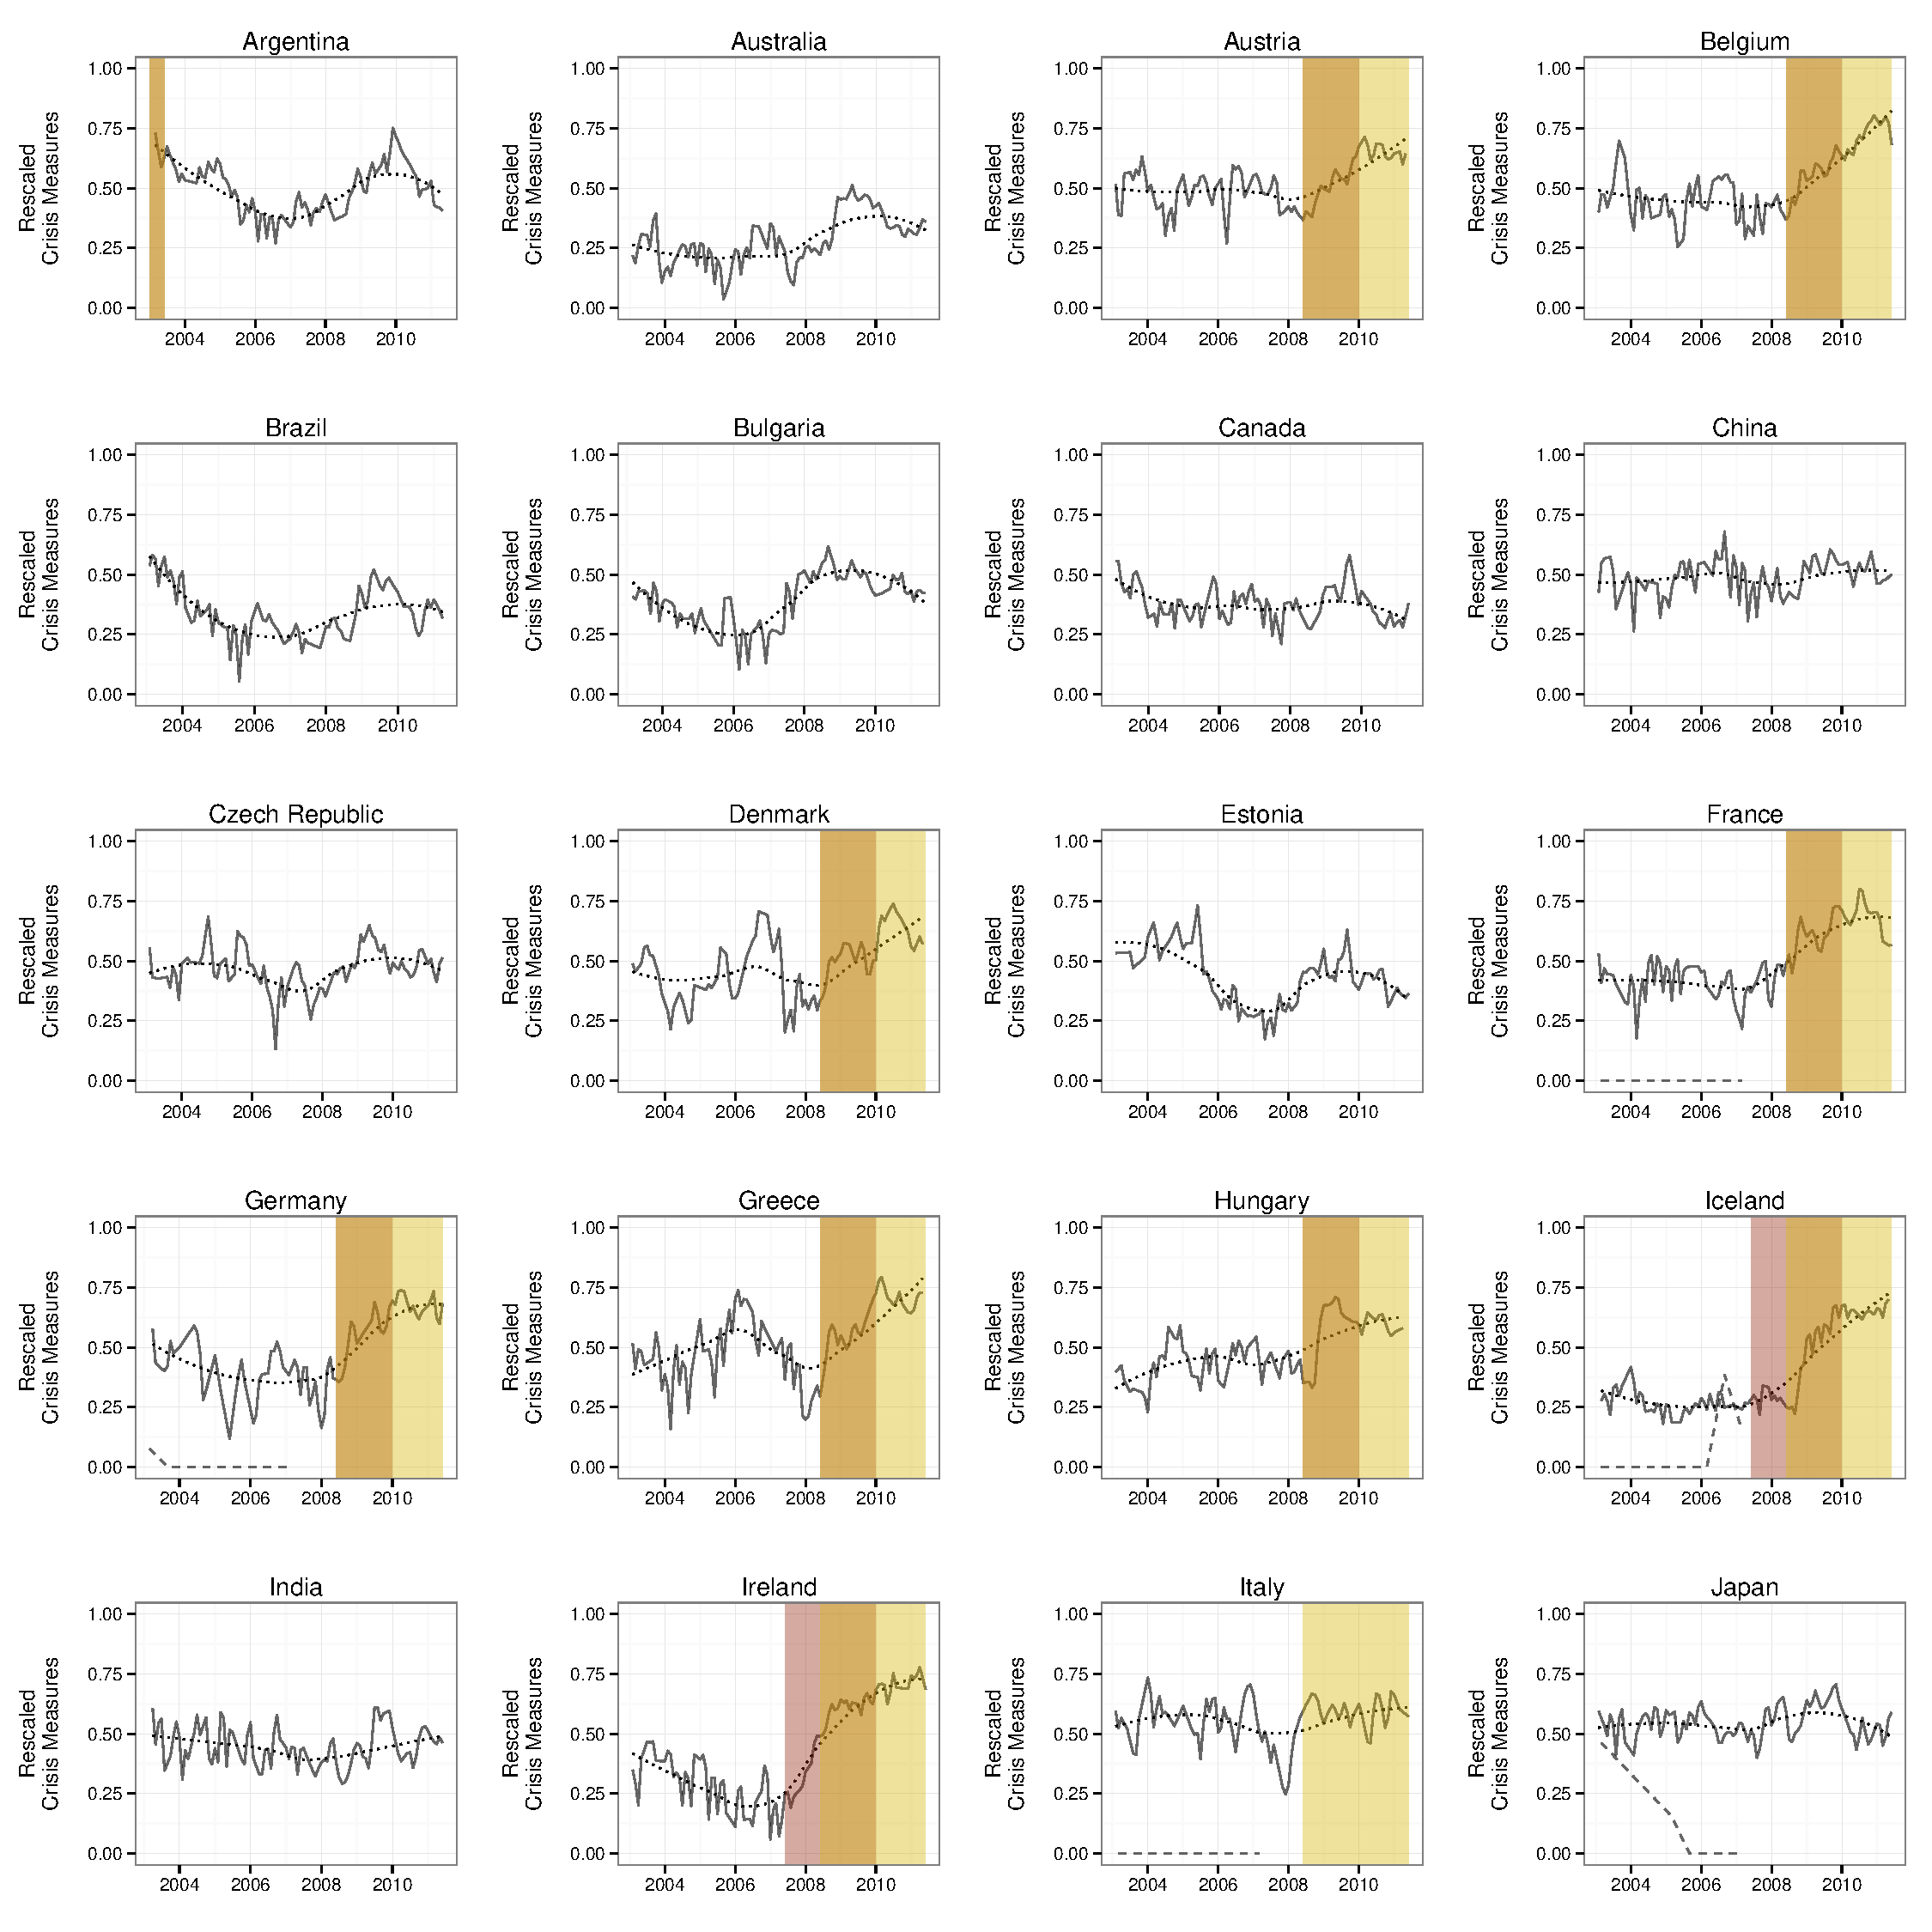
\includegraphics[scale=0.23]{figures/compare_to_lv_rr.pdf}
    \end{center}

}

\frame{
    \frametitle{Credit provision vs. financial market stress}

    Why credit provision stress, not financial market stress more broadly?

    \vspace{1cm}

    In general, {\large{\textbf{politicians care}}} about financial market stress to the extent that it {\large{\textbf{hits credit provision to the real economy}}}.

}

\frame{
    \frametitle{Interactions}

    Hypothesise that election variables have a {\large{\textbf{larger impact}}} on revisions during {\large{\textbf{high stress}}}.

    \begin{center}
        so
    \end{center}

    Focus on {\textbf{interactions}} between election variables and FinStress.
}

\frame{
    \frametitle{Right-hand side}

    {\large{Also:}}

    \begin{itemize}
        \item Years since publication

        \item Eurozone membership

        \item Exchange rate (vs. USD)

        \item Absolute gross debt \& deficit levels (2015 vintage)

        \item Country-varying intercepts
    \end{itemize}

}

\section{Empirics: (Preliminary) Results}

\frame{
\begin{figure}
    \caption{Marginal Effect of Election Timing (years to election) at Various Levels of Financial Market Stress on \textbf{Debt} Revisions}
    \label{me_finstress_elect}

    \begin{center}
        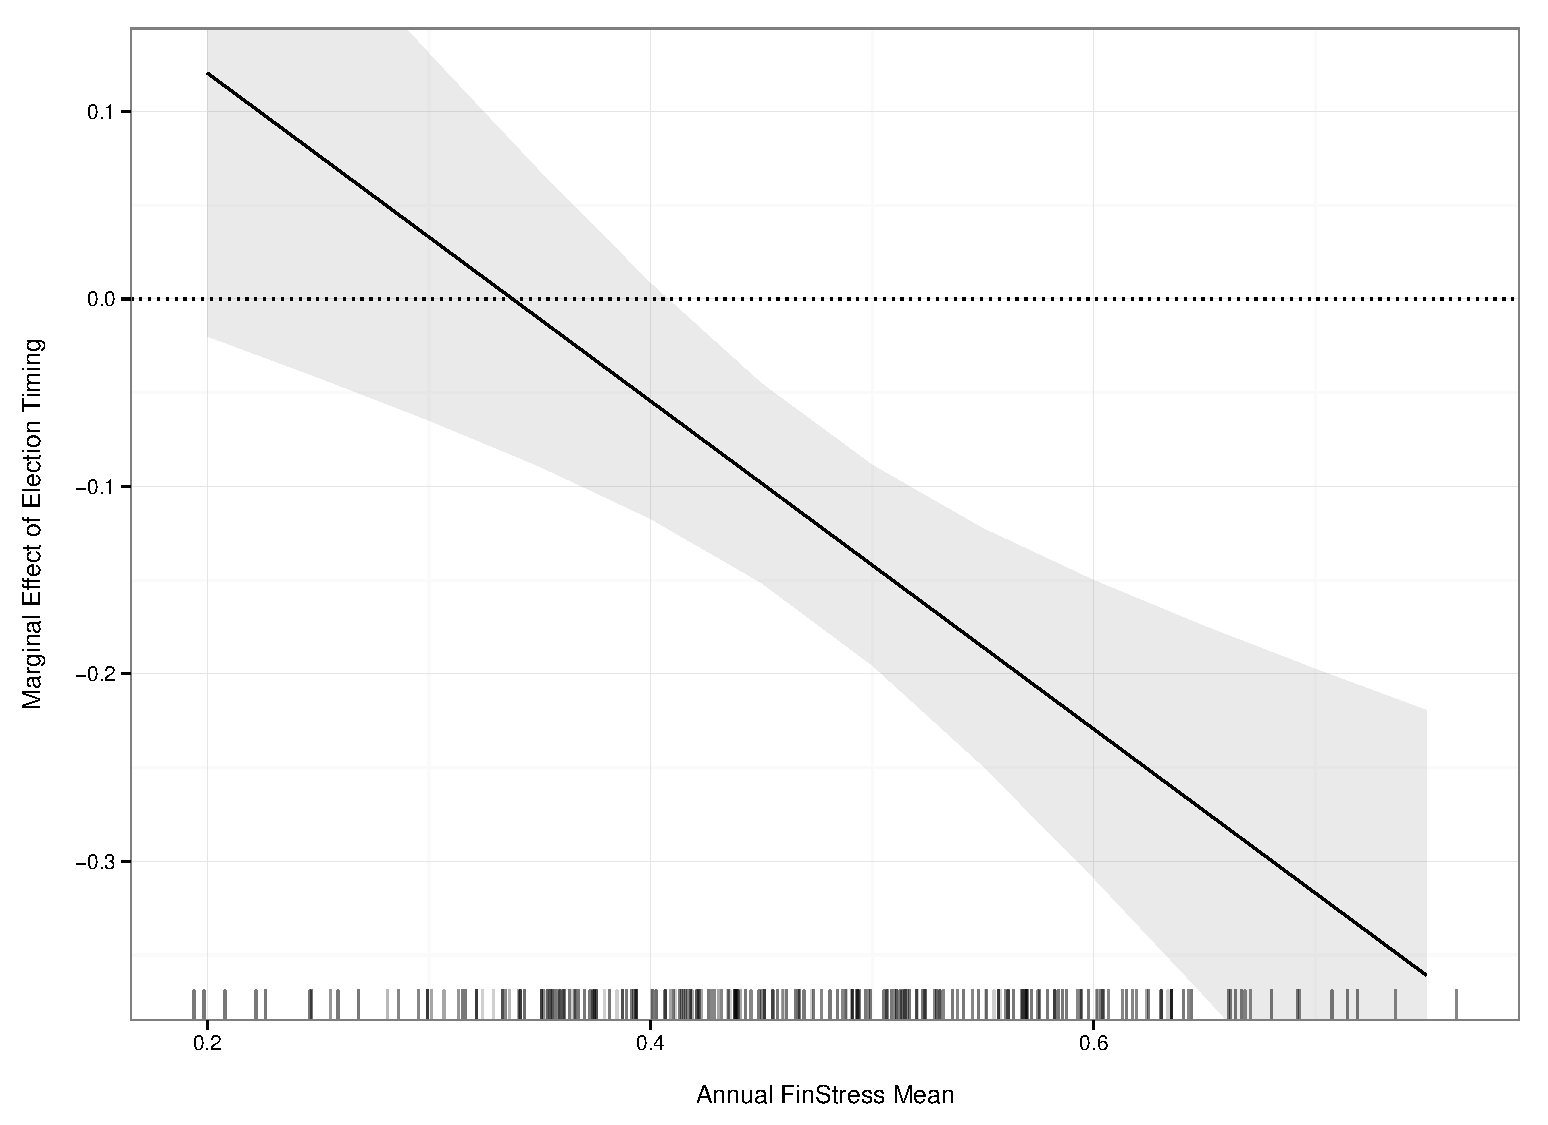
\includegraphics[scale=0.4]{figures/finstress_elect_me.pdf}
    \end{center}

\end{figure}

}

\frame{

\begin{figure}
    \caption{Marginal Effect of an Endogenous Election at Various Levels of Financial Market Stress on \textbf{Debt} Revisions}
    \label{me_finstress_endog_elect}

    \begin{center}
        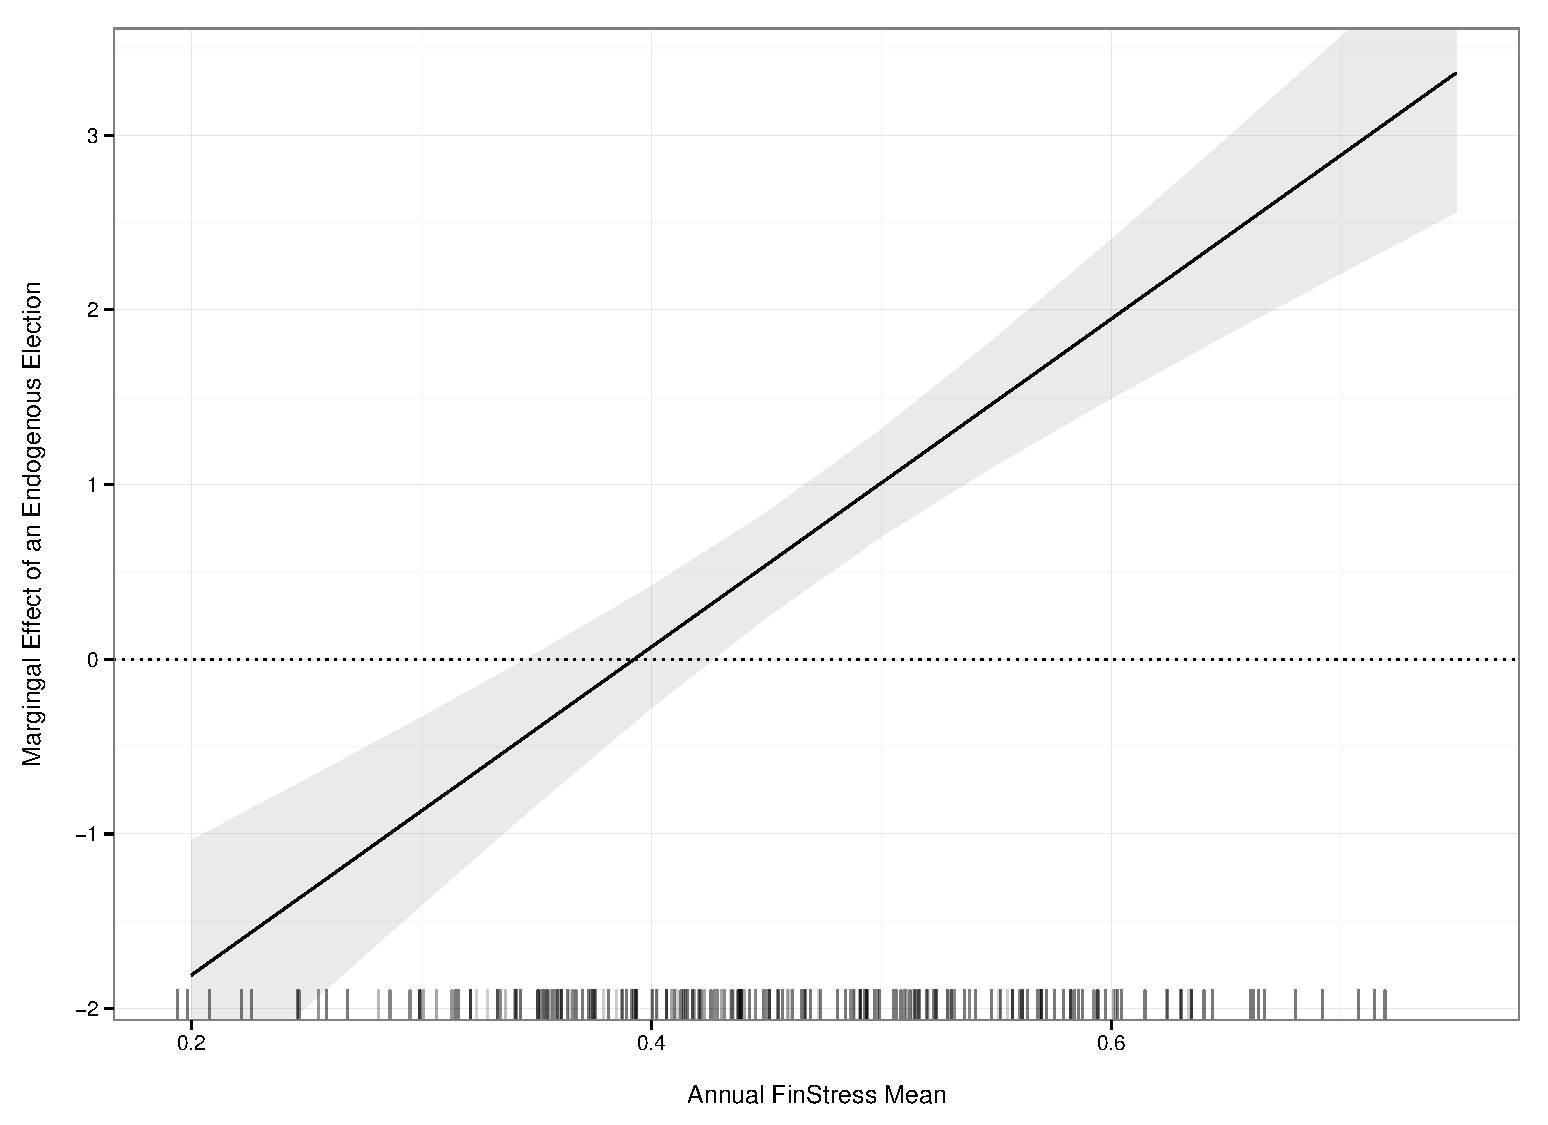
\includegraphics[scale=0.4]{figures/finstress_endog_elect_me.pdf}
    \end{center}

\end{figure}

}

\frame{

\begin{figure}
	\caption{Predicted \textbf{Debt} Revisions in Four Years After Publication for Years with Different Election Types/Non-election Years}
    \label{country_predict_debt_required}
    \begin{center}
    	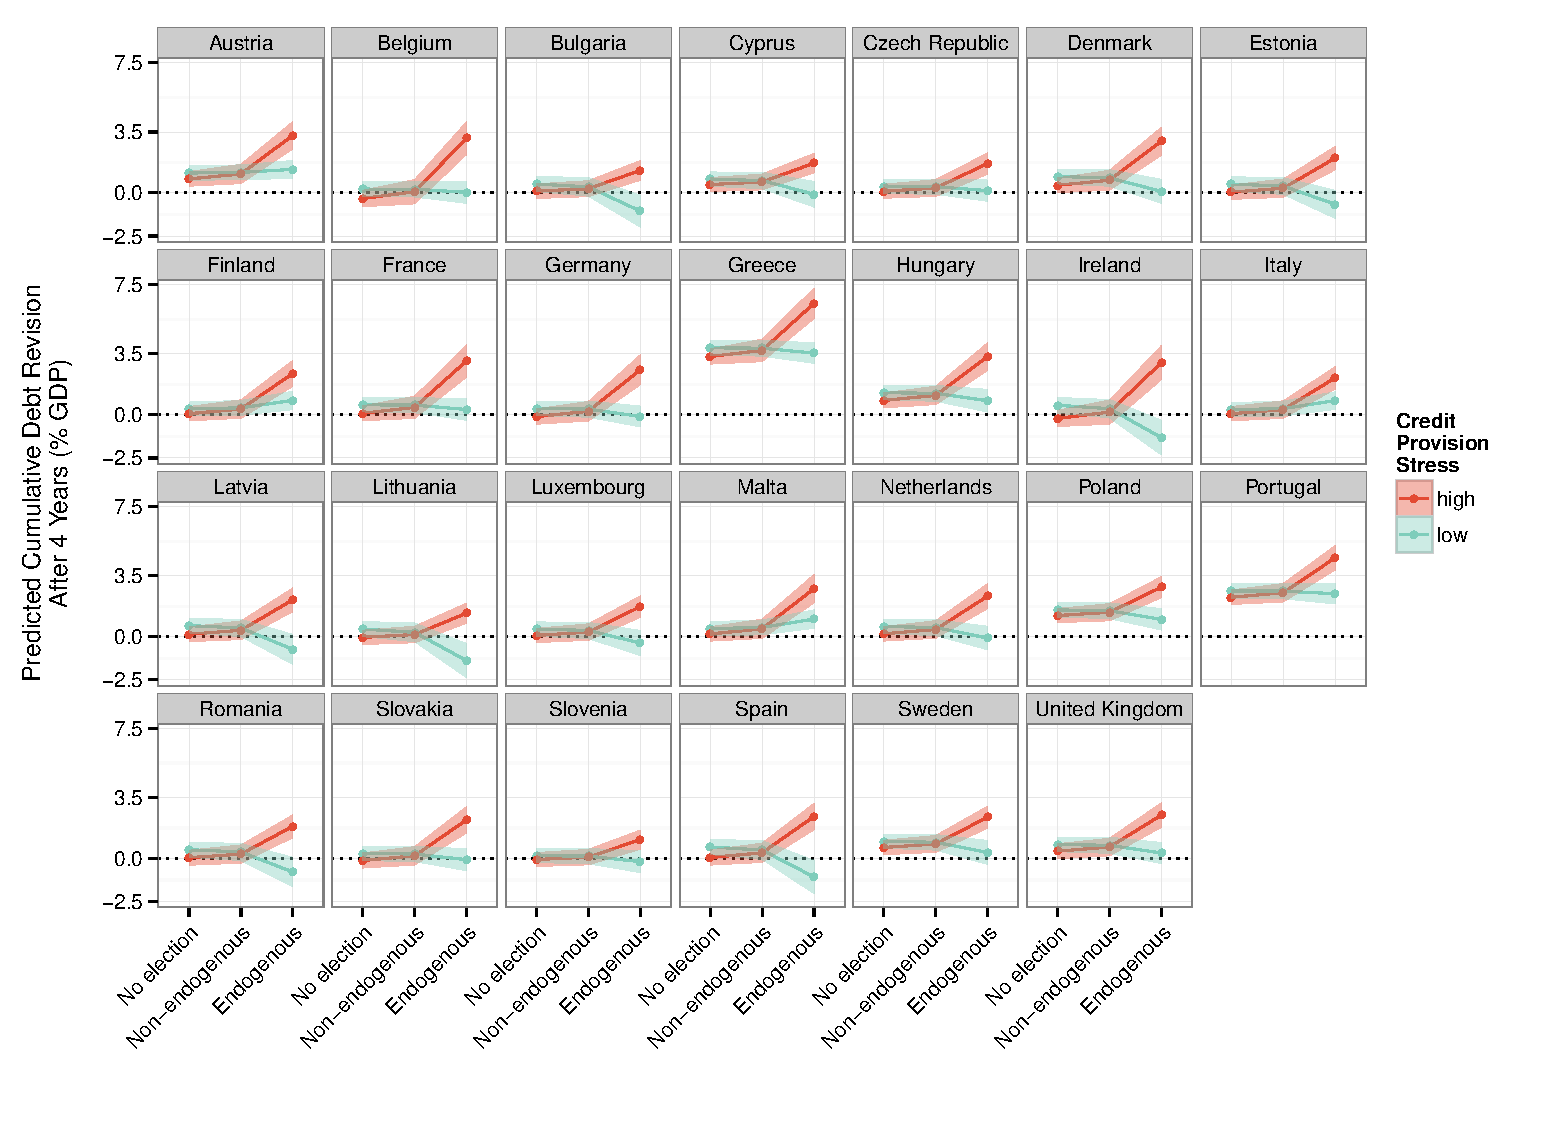
\includegraphics[scale=0.4]{figures/country_predict_required.pdf}
    \end{center}

\end{figure}

}

\frame{

\begin{figure}
    \caption{Marginal Effect of a Non-Endogenous Election at Various Levels of Financial Market Stress on \textbf{Deficit} Revisions}
    \label{me_finstress_non_endog_deficit}
    \begin{center}
        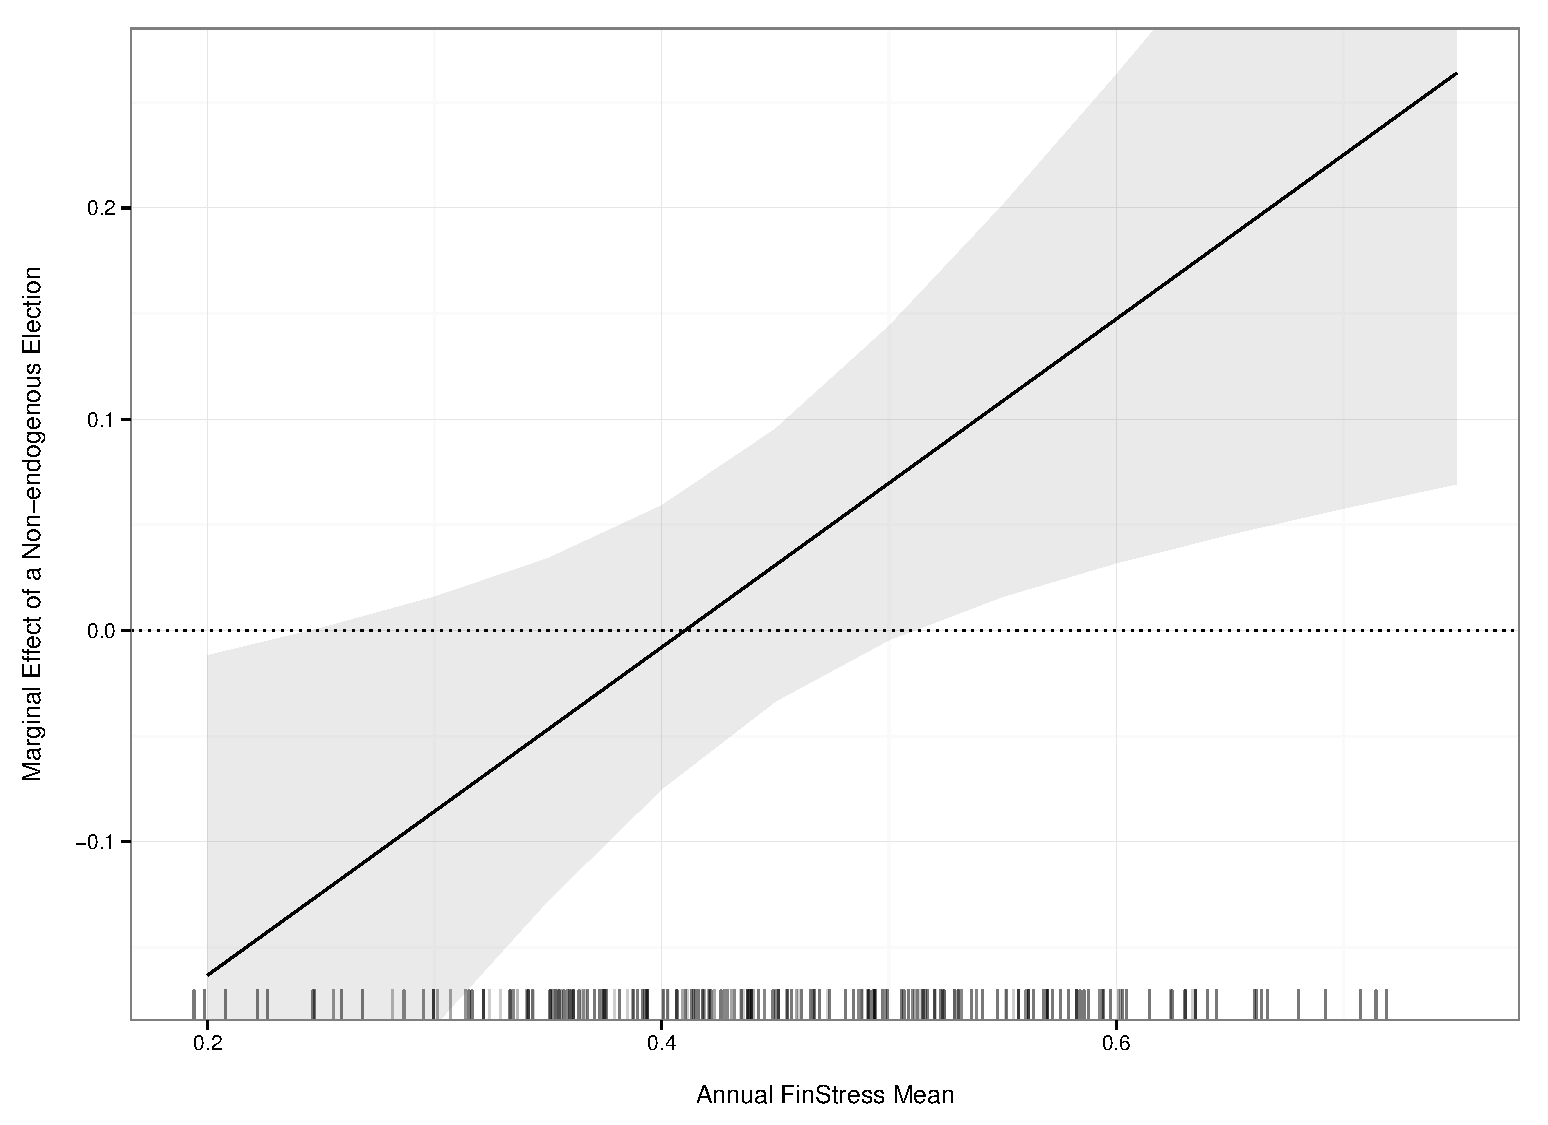
\includegraphics[scale=0.4]{figures/finstress_non_endog_deficit_me.pdf}
    \end{center}

\end{figure}

}


\section{Conclusion/Still to do}

\frame{
    \frametitle{To-Do: Empirical}

    Omitted variables?:

    \begin{itemize}
        \item independence of national accounting agency.

        \item SGP enforcement actions (not just eurozone membership)

        \item Others?
    \end{itemize}

    \vspace{1cm}

    Model choice: normal linear regression with many 0s?

}

\frame{
    \frametitle{To-Do: Theoretical}
    \begin{itemize}
        \item Understand interaction between scheduled elections and FinStress on deficit revisions.
    \end{itemize}

}

\end{document}
